\documentclass{article}
\input{tex/00_preambule.tex}

\author{Artur Radwański}
\title{Interpolacja funkcjami sklejanymi 2 i 3 stopnia}
\setDepartment{Wydział Informatyki}
\setSupervisor{Grupa 4}

\begin{document}

\maketitle


\linespread{1.3}
\selectfont

\section{System}
\begin{itemize}
    \item Procesor: AMD Ryzen 7 9800x3d
    \item System operacyjny: 6.19.9-arch1-1 (Linux)
    \item Język programowania: c++23
    \item Kompilator: gcc version 15.2.1 20260209 (GCC) 
\end{itemize}


\section{Zadanie}
\subsection{Cel}
Celem niniejszego opracowania jest analiza metod interpolacji funkcjami sklejanymi (splajnami) drugiego oraz trzeciego stopnia. W przeciwieństwie do
interpolacji wielomianowej globalnej, funkcje sklejane pozwalają na uniknięcie efektu Rungego poprzez konstrukcję lokalnych wielomianów niskiego stopnia w
każdym przedziale $[x_i, x_{i+1}]$. Zbadano skuteczność takiego podejścia na podstawie funkcji:
\[f(x) = -2x\sin(2(x-1))\hspace{5ex}  x\in[-2\pi+1,3\pi+1]\]



\subsection{Realizacja}

W celu zbadania właściwości numerycznych wybranych metod interpolacji, zaimplementowano środowisko testowe w języku C++, pozwalające na automatyczne porównanie
wyników dla zmiennej liczby węzłów $n \in [5, 50]$. Proces badawczy zrealizowano w następujących krokach:

\begin{enumerate}
    \item \textbf{Generowanie węzłów interpolacji:} Dla każdej liczby węzłów interpolacji wyznaczono zestaw punktów równoodległych w przedziale $[a, b]$:
    

    \item \textbf{Analiza błędów:} Dla każdego zestawu danych przeprowadzono próbkowanie w $k=1000$ punktach kontrolnych rozmieszczonych równomiernie. Jako miary dokładności przyjęto:
    \begin{itemize}
        \item \textbf{Błąd średnio-kwadratowy ($MSE$):} dający obraz ogólnego dopasowania funkcji na całym przedziale.
        
        \begin{center}
        \begin{Large}
            \[E_{sqr} = \frac{\sqrt{\sum_{i}^{k}(P(x_{i}) - f(x_{i}))^{2}}}{k}\]
        \end{Large}
        \end{center}  
        
        
        Gdzie $P(x)$ to wielomian interpolujący, a $x_{i}$ to kolejne punkty kontrolne 
        \item \textbf{Błąd maksymalny ($E_{max}$):} służy głównie do zaobserwowania jaki błąd da interpolacja w przypadku pesymistycznym.
        
        \begin{center}
        \begin{Large}
            \[E_{max}=\max_{i\in[1,k]}(x_{i})\]
        \end{Large}
        \end{center}
        
        Gdzie $x_{i}$ to kolejne punkty kontrolne
    \end{itemize}
\end{enumerate}

\subsection{Interpolacja splajnami trzeciego stopnia}

Splajn trzeciego stopnia w $i$-tym przedziale definiujemy jako wielomian:
\begin{equation}
S_i(x) = a_i + b_i(x - x_i) + c_i(x - x_i)^2 + d_i(x - x_i)^3
\end{equation}
Wyznaczenie współczynników opiera się na wyliczeniu drugich pochodnych w węzłach o współrzędnych $(x_{i}, y_{i})$. Relację między nimi dla węzłów wewnętrznych $i = 1, \dots, n-2$ opisuje układ równań:
\begin{equation}
h_{i-1}\sigma_{i-1} + 2(h_{i-1} + h_i)\sigma_i + h_i\sigma_{i+1} = 6 \left( \frac{y_{i+1}-y_i}{h_i} - \frac{y_i-y_{i-1}}{h_{i-1}} \right)
\end{equation}
gdzie $h_i = x_{i+1} - x_i$ jest krokiem między węzłami, a $\sigma_i = S''(x_i)$. Układ ten tworzy macierz trójdiagonalną, którą rozwiązujemy efektywnie algorytmem Thomasa.
Następnie obliczamy kolejne współczynniki wielomianów korzystając z następujących wzorów:
\begin{itemize}
    \begin{Large}
    \item $a_i = y_i$
    \item $b_i = \frac{y_{i+1} - y_{i}}{h_i} - h_i \frac{\sigma_{i+1} + 2\sigma_{i}}{6}$
    \item $c_i = \frac{\sigma_i}{2}$
    \item $d_i = \frac{\sigma_{i+1} - \sigma_i}{6h_i}$
    \end{Large}
\end{itemize}

Wykresy ze splajnami 3. stopnia podpisane są "splajn sześcienny".

\subsection{Interpolacja splajnami drugiego stopnia }

Wielomian w przedziale ma postać $S_i(x) = a_i(x-x_i)^2 + b_i(x-x_i) + c_i$ $i=0...n-2 $. Współczynniki wyznaczane są rekurencyjnie przy zachowaniu ciągłości funkcji oraz jej pierwszej pochodnej ($C^1$):
\begin{itemize}
    \begin{Large}
    \item $c_i = y_i$
    \item $a_i = \frac{y_{i+1} - y_i - b_i h_i}{h_i^2}$
    \item $b_{i+1} = 2a_i h_i + b_i$
    \end{Large}
\end{itemize}

Wykresy ze splajnami 3. stopnia podpisane są "splajn kwadratowy".

\subsection{Warunki brzegowe}

Ze względu na to, że liczba niewiadomych w splajnach jest większa niż liczba równań wynikających z warunków ciągłości, konieczne jest narzucenie warunków brzegowych.

\subsubsection{Splajn naturalny}
Zakłada, że funkcja na krańcach przedziału "prostuje się", co odpowiada zerowaniu się odpowiednich pochodnych:
Dla funkcji sklejanych 3. stopnia zakładamy, że zerują się ich drugie pochodne dla pierwszego i ostatniego węzła ($\sigma_0 = \sigma_{n-1} = 0$), natomiast dla splajnów kwadratowych
przyjmujemy, że zeruje się jego pochodna w pierwszym węźle ($b_0$ = 0).


W tabelach i wykresach ten warunek opisany jest jako "Naturalny".

\subsubsection{Znane pochodne}
Stosowany, gdy posiadamy informację o nachyleniu lub krzywiźnie funkcji na brzegach. W przypadku splajnów 3. stopnia narzucamy wartości $\sigma_0 = 8,01$ oraz
$\sigma_{n-1} = -7,99$ , natomiast w splajnach 2. stopnia zadajemy wartość pierwszej pochodnej $b_0 = 21,14 $. (Wzory na pochodne wyznaczone analitycznie, następnie
wynik zaokrąglony do dwóch miejsc po przecinku).

W tabelach i wykresach opisany jako "Pochodna".

\subsubsection{Warunek `Not-a-knot`}
Wymusza ciągłość wyższych pochodnych w pierwszym i ostatnim węźle wewnętrznym, co sprawia, że pierwsze dwa oraz ostatnie dwa segmenty są opisane tym samym wielomianem.
\begin{itemize}
    \item \textbf{Stopień 3:} $\sigma_0(x_1) = \sigma_1(x_1)$ oraz $\sigma_{n-2}(x_{n-2}) = \sigma_{n-1}{(x_{n-2})}$ (ciągłość trzeciej pochodnej).
    \item \textbf{Stopień 2:} $S''_0(x_1) = S''_1(x_1)$ (ciągłość drugiej pochodnej).
\end{itemize}

W tabelach i wykresach opisany jako "Not-a-knot".
\section{Wyniki}
\begin{table}[H]
\centering
\begin{tabular}{|c|cc|cc|cc|}
\hline
\textbf{n} & \multicolumn{2}{c|}{\textbf{Naturalny}} & \multicolumn{2}{c|}{\textbf{Pochodna}} & \multicolumn{2}{c|}{\textbf{Not-a-knot}} \\ \cline{2-7}
& \textbf{MSE} & \textbf{MAX} & \textbf{MSE} & \textbf{MAX} & \textbf{MSE} & \textbf{MAX} \\ \hline
5  & 3.06e-01 & 27.0858 & 3.31e-01 & 32.0226 & 3.16e-01 & 29.7276 \\
10 & 2.53e-01 & 25.1446 & 2.49e-01 & 24.0032 & 2.81e-01 & 28.9762 \\
15 & 4.10e-02 & 4.4579  & 4.05e-02 & 3.9858  & 2.95e-02 & 3.0137  \\
20 & 8.36e-03 & 1.0434  & 8.44e-03 & 1.0329  & 1.95e-02 & 3.3172  \\
25 & 2.84e-03 & 0.4011  & 3.00e-03 & 0.4954  & 1.01e-02 & 1.9893  \\
30 & 1.31e-03 & 0.2069  & 1.46e-03 & 0.2956  & 5.50e-03 & 1.2079  \\
35 & 7.29e-04 & 0.1266  & 8.57e-04 & 0.1989  & 3.23e-03 & 0.7750  \\
40 & 4.58e-04 & 0.0862  & 5.61e-04 & 0.1445  & 2.03e-03 & 0.5238  \\
45 & 3.12e-04 & 0.0629  & 3.94e-04 & 0.1101  & 1.34e-03 & 0.3699  \\
50 & 2.25e-04 & 0.0483  & 2.92e-04 & 0.0870  & 9.31e-04 & 0.2713  \\ \hline
\end{tabular}

\caption{Zbiorcze zestawienie błędów MSE i MAX dla interpolacji splajnami 3. stopnia (n=5 do n=50).}
\label{tab:cubic_full}
\end{table}

\begin{table}[H]
\centering

\begin{tabular}{|c|cc|cc|cc|}
\hline
\textbf{n} & \multicolumn{2}{c|}{\textbf{Natural}} & \multicolumn{2}{c|}{\textbf{Derivative}} & \multicolumn{2}{c|}{\textbf{Not-a-knot}} \\ \cline{2-7}
& \textbf{MSE} & \textbf{MAX} & \textbf{MSE} & \textbf{MAX} & \textbf{MSE} & \textbf{MAX} \\ \hline
5  & 3.48e-01 & 35.9053 & 4.84e-01 & 31.9121 & 3.33e-01 & 34.5997 \\
10 & 5.12e-01 & 49.5485 & 4.28e-01 & 40.3401 & 5.33e-01 & 51.0435 \\
15 & 2.65e-01 & 18.5044 & 1.41e-01 & 12.5858 & 1.80e-01 & 14.5191 \\
20 & 1.33e-01 & 7.0244  & 3.49e-02 & 2.6788  & 3.05e-02 & 2.4627  \\
25 & 9.38e-02 & 4.5029  & 1.50e-02 & 1.1139  & 6.33e-03 & 0.6559  \\
30 & 7.34e-02 & 3.4064  & 7.78e-03 & 0.5472  & 4.40e-03 & 0.4053  \\
35 & 6.07e-02 & 2.7163  & 4.63e-03 & 0.3207  & 4.21e-03 & 0.2907  \\
40 & 5.20e-02 & 2.3189  & 2.96e-03 & 0.1935  & 3.62e-03 & 0.2273  \\
45 & 4.55e-02 & 2.0084  & 2.03e-03 & 0.1365  & 2.95e-03 & 0.1698  \\
50 & 4.05e-02 & 1.7766  & 1.44e-03 & 0.0914  & 2.39e-03 & 0.1333  \\ \hline
\end{tabular}
\caption{Zbiorcze zestawienie błędów MSE i MAX dla interpolacji splajnami 2. stopnia (n=5 do n=50).}
\label{tab:quadratic_full}
\end{table}

\begin{figure}[h]
    \centering
    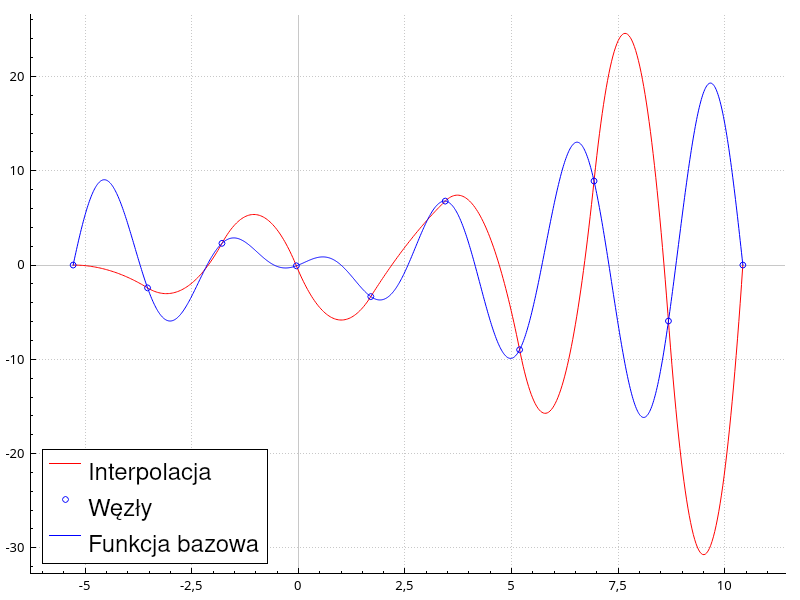
\includegraphics[width=0.8\textwidth]{img/n=10QNatural.png}
    \caption{n=10 splajn kwadratowy, Naturalny}
    \label{fig:quadratic_n=10}
\end{figure}


Jak widać w tabelach \ref{tab:cubic_full} i \ref{tab:quadratic_full} błąd interpolacji splajnami stale się zmniejsza razem ze wzrostem liczby węzłów interpolacji.
Wyjątkiem od tej zależności jest wiersz dla n=10 dla funkcji sklejanych 2 stopnia, jednak na rysunku \ref{fig:quadratic_n=10} możemy zaobserwować, że jest to
jedynie efekt niefortunnego umieszczenia 3 ostatnich węzłów interpolacji przez które splajn zaczyna oscylować "odwrotnie" niż funkcja bazowa, co generuje duży błąd. 
Splajny 3. stopnia przybliżają funkcję znacznie lepiej niż splajny stopnia 2. Dla małej liczby węzłów (n=5) różnica jest niewielka, jednak w miarę zwiększania
n, relatywna różnica się zwiększa, dla n = 50 osiąga 1 lub 2 rzędy wielkości w zależności od przyjętych warunków brzegowych.



% \begin{figure}[h]
%     \centering
%     \begin{subfigure}{0.6\textwidth}
%         \caption{n=15 splajn kwadratowy, Pochodna}
%         \label{fig:quadratic_derivative}
%         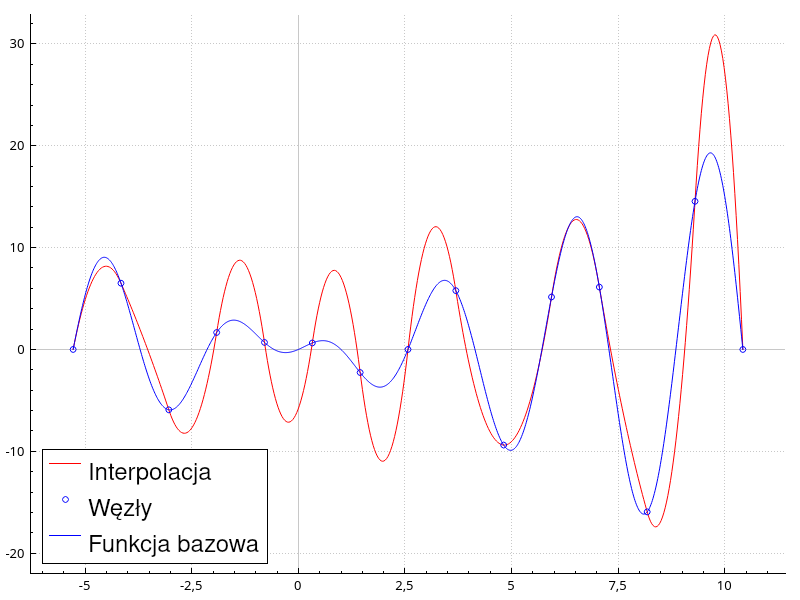
\includegraphics[width=\textwidth]{img/n=15QDeriv.png}
%     \end{subfigure}
%     \begin{subfigure}{0.6\textwidth}
%         \caption{n=15 splajn kwadratowy, Naturalny}
%         \label{fig:quadratic_natural}
%         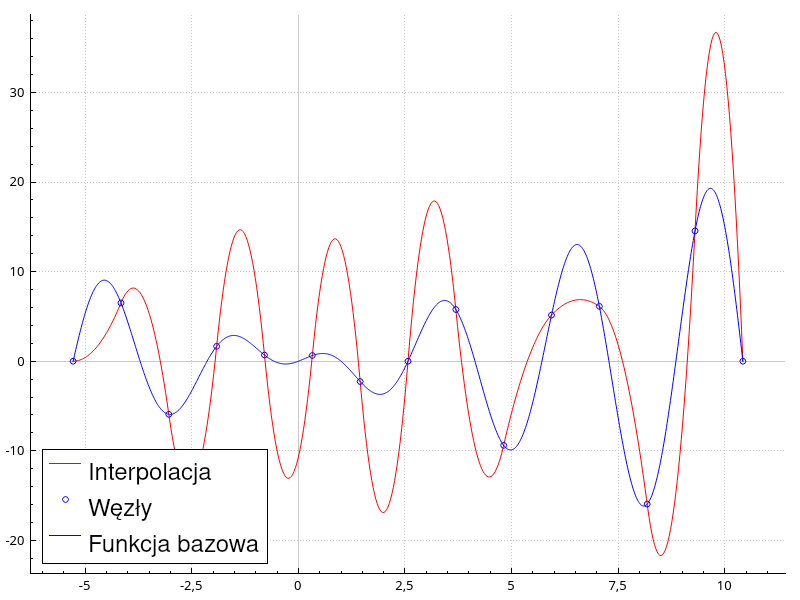
\includegraphics[width=\textwidth]{img/n=15QNatural.png}
%     \end{subfigure}
%     \begin{subfigure}{0.6\textwidth}
%         \caption{n=15 splajn kwadratowy, Not-a-Knot}
%         \label{fig:quadratic_knot}
%         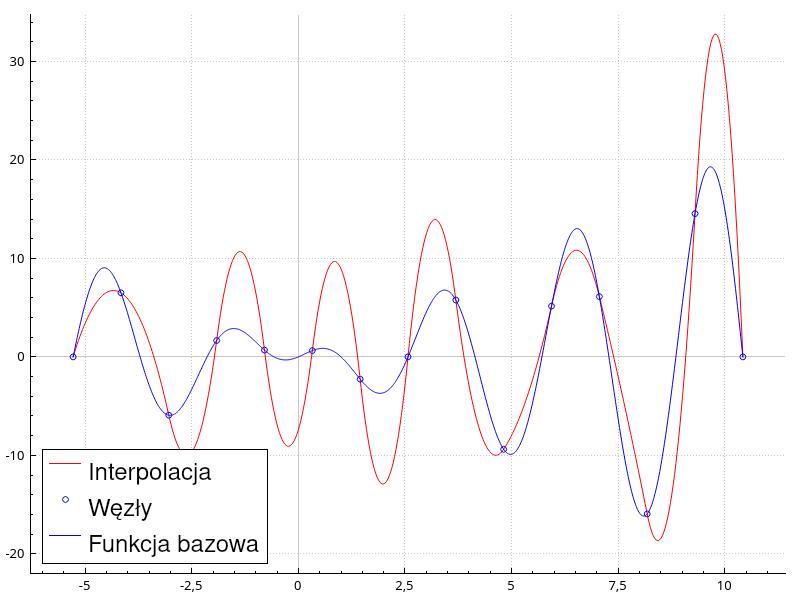
\includegraphics[width=\textwidth]{img/n=15QKnot.png}
%     \end{subfigure}
% \end{figure}


\subsection{Warunki brzegowe w funkcjach sklejanych drugiego stopnia}
\begin{figure}[h]
    \centering
    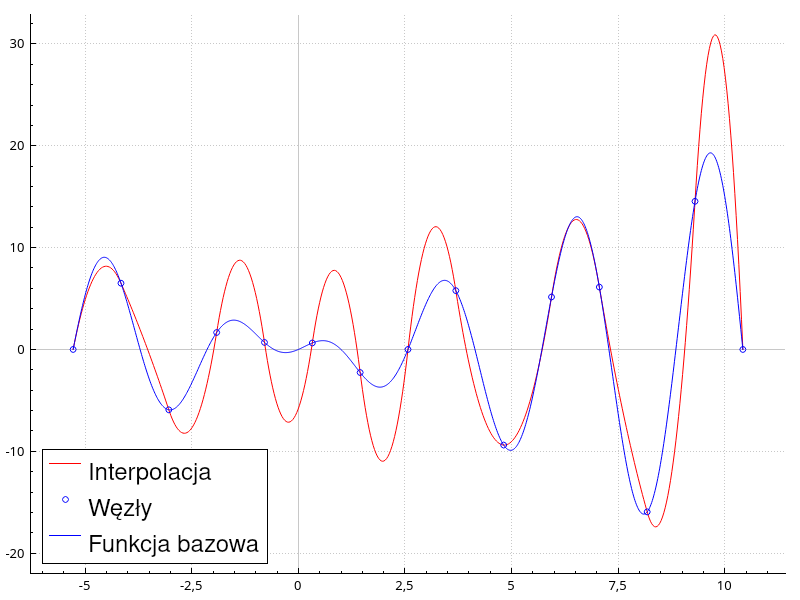
\includegraphics[width=0.8\textwidth]{img/n=15QDeriv.png}
    \caption{n=15 splajn kwadratowy, Pochodna}
    \label{fig:quadratic_derivative}
\end{figure}

\begin{figure}[H]
    \centering
    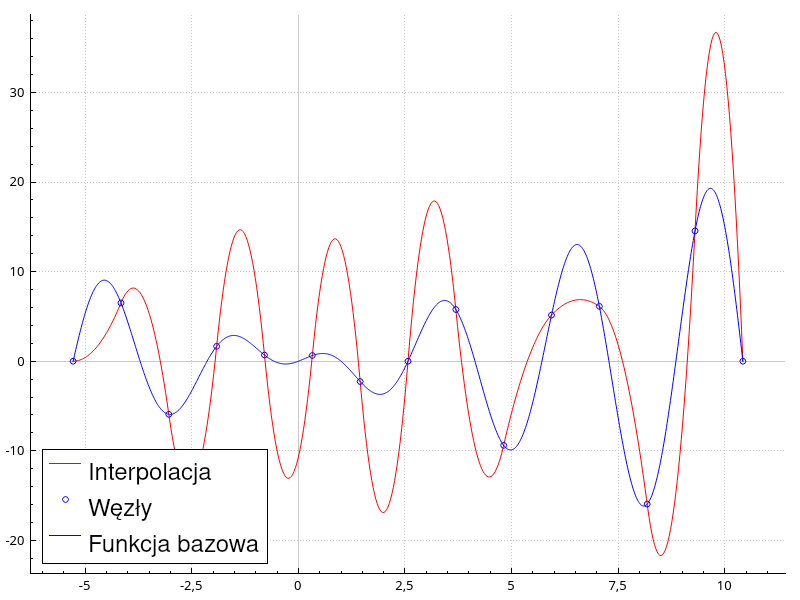
\includegraphics[width=0.8\textwidth]{img/n=15QNatural.png}
    \caption{n=15 splajn kwadratowy, Naturalny}
    \label{fig:quadratic_natural}
\end{figure}

W tabeli \ref{tab:quadratic_full} możemy zauważyć, że interpolacja generuje największy błąd dla splajnu naturalnego, trochę lepiej przy zastosowaniu warunku
"Not-a-Knot", a najlepiej kiedy znamy wartość drugiej pochodnej funkcji bazowej. Jest to wynik zgodny z intuicją ponieważ, wykorzystanie dodatkowej informacji
o interpolowanej funkcji jako warunku brzegowego powinno polepszać interpolację. Warunek "Not-a-Knot" próbuje
wykorzystać dostępne informacje o funkcji żeby stworzyć dodatkowe równanie, natomiast w przypadku sztywnego ustawienia drugiej pochodnej na 0, wprowadzamy
sztuczny warunek który nie ma musi mieć pokrycia w rzeczywistości i daje różne rezultaty w zależności od badanej funkcji.


\begin{figure}[H]
    \centering
    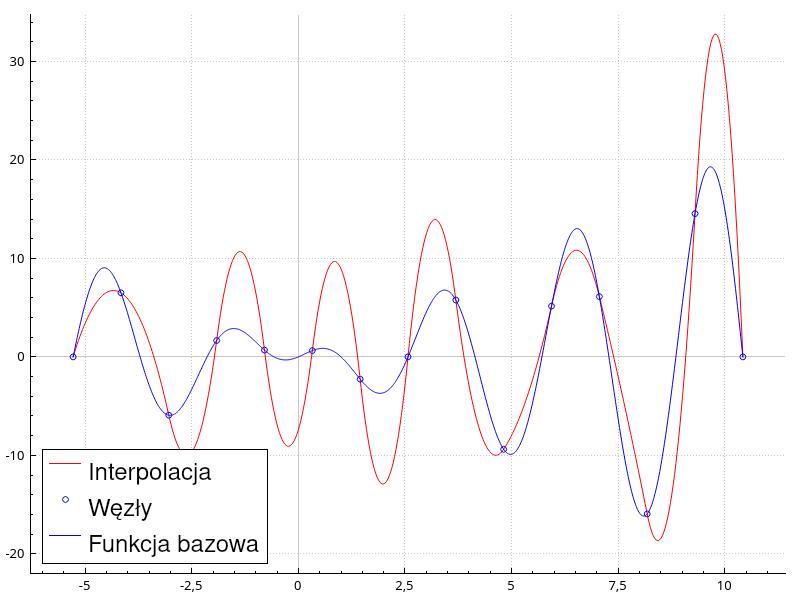
\includegraphics[width=0.8\textwidth]{img/n=15QKnot.png}
    \caption{n=15 splajn kwadratowy, Not-A-Knot}
    \label{fig:quadratic_knot}
\end{figure}

Rysunki \ref{fig:quadratic_derivative}, \ref{fig:quadratic_natural} i \ref{fig:quadratic_knot}  przedstawiają funkcje sklejane
wygenerowane dla tych samych węzłów z różnymi warunkami brzegowymi. Wybrano n=15, ponieważ różnica między warunkami brzegowymi zanika wraz ze
wzrostem liczby węzłów, a dla n=15 wciąż jest widoczna, a jednocześnie dla takiej liczby węzłów funkcja interpolująca zaczyna optycznie przypominać funkcję bazową.


\subsection{Warunki brzegowe w funkcjach sklejanych drugiego stopnia}

Z tabeli \ref{tab:cubic_full} wynika, że dla splajnów 3. stopnia nie można w oczywisty sposób zdecydować który z warunków brzegowych jest najlepszy.
Warunki brzegowe mają mniejszy wpływ na przebieg splajnów wyższych stopni. Warunki brzegowe które teoretycznie powinny być lepsze ponieważ robią użytek
z dodatkowych informacji o funkcji bazowej sprawują się na podobnym poziomie co splajn naturalny. Na rysunkach \ref{fig:cubic_natural}, \ref{fig:cubic_derivative}
oraz \ref{fig:cubic_knot} można zobaczyć, że już dla n=15 zmiana warunków brzegowych powoduje jedynie nieznaczne zmiany przy krawędziach badanego przedziału.

\begin{figure}[H]
    \centering
    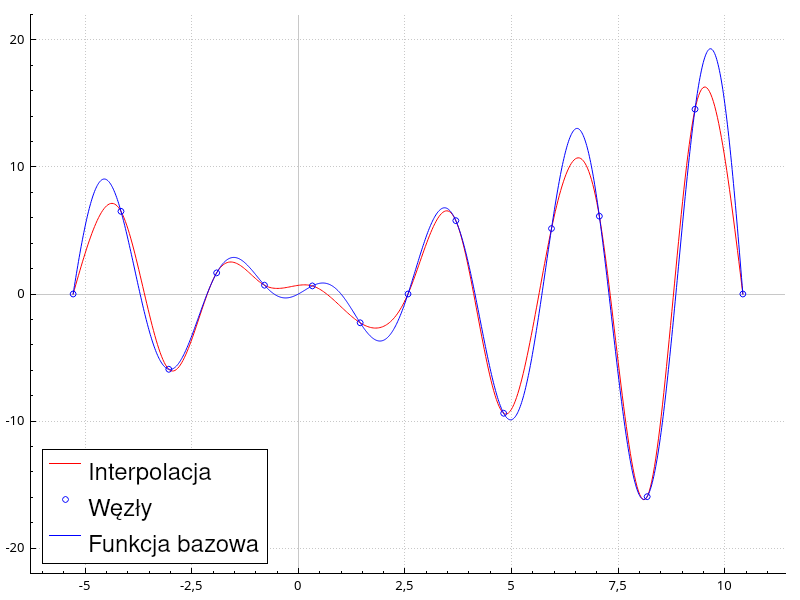
\includegraphics[width=0.8\textwidth]{img/n=15CNatural.png}
    \caption{n=15 splajn sześcienny, Naturalny}
    \label{fig:cubic_natural}
\end{figure}

\begin{figure}[H]
    \centering
    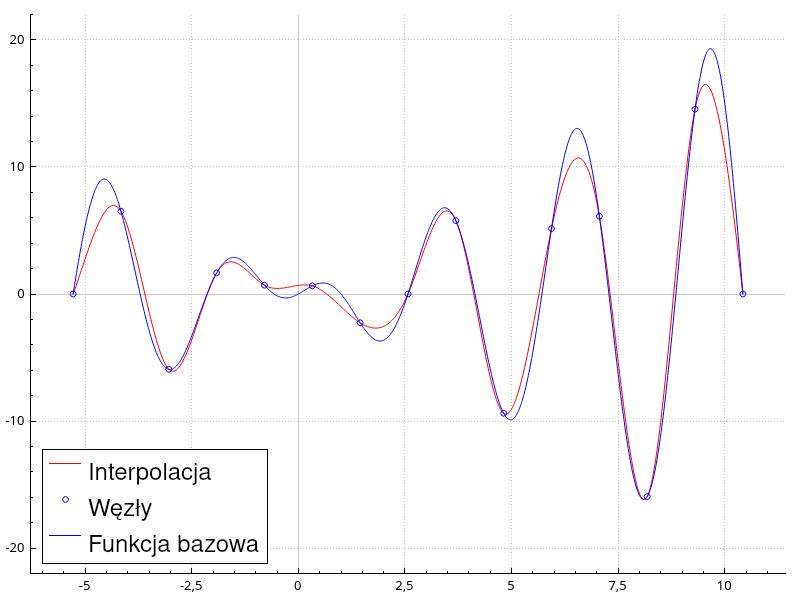
\includegraphics[width=0.8\textwidth]{img/n=15CDeriv.png}
    \caption{n=15 splajn sześcienny, Pochodna}
    \label{fig:cubic_derivative}
\end{figure}

\begin{figure}[H]
    \centering
    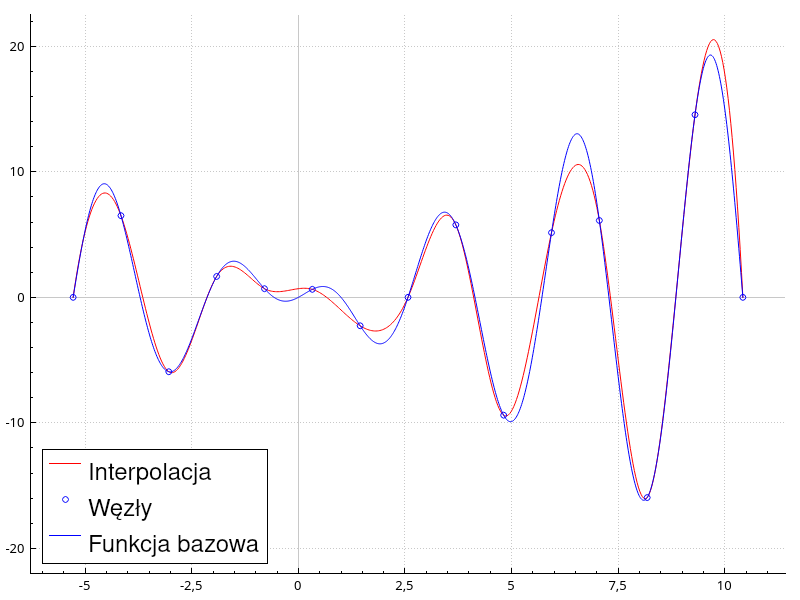
\includegraphics[width=0.8\textwidth]{img/n=15CKnot.png}
    \caption{n=15 splajn sześcienny, Not-a-Knot}
    \label{fig:cubic_knot}
\end{figure}

\section{Wnioski}
W przypadku interpolacji funkcjami sklejanymi drugiego stopnia, warto zwrócić uwagę na warunek brzegowy. Jeśli jest możliwe obliczenie drugiej pochodnej
funkcji bazowej najlepiej jest jej użyć do interpolacji, a w przeciwnym razie zaimplementować warunek "Not-a-Knot". W przypadku splajnów 3. stopnia warunki brzegowe
nie odgrywają aż tak dużej roli w zmniejszeniu błędu interpolacji. W tym przypadku lepsze efekty w zmniejszeniu błędu daje zwiększanie liczby węzłów interpolacji.
Porównując funkcje sklejane między sobą, splajny 3. stopnia przybliżają funkcję bazową znacznie lepiej. 

\end{document}